\chapter{Capa de Negocio}
\section{Introducción}
contenido...
\newpage
\section{Punto de Vista de Organización}
\subsection{Modelo}
The Organization viewpoint focuses on the (internal) organization of a company, a department, a network of companies, or of another organizational entity. It is possible to present models in this viewpoint as nested block diagrams, but also in a more traditional way, such as organizational charts. The Organization viewpoint is very useful in identifying competencies, authority, and responsibilities in an

\begin{figure}[h!]
	\centering
	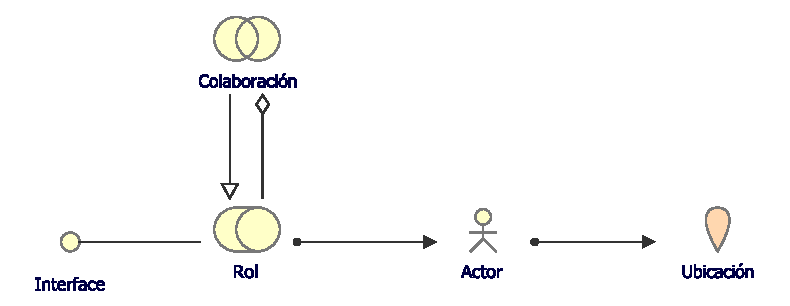
\includegraphics[width=1\linewidth]{ARQUITECTURA/imgs/MOrganizacion}
	\caption{Modelo de Ogranización}
\end{figure}


\newpage
\subsection{Caso de Estudio}

\begin{figure}[h!]
	\centering
	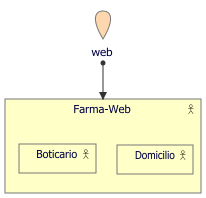
\includegraphics[width=.5\linewidth]{ARQUITECTURA/imgs/COrganizacion}
	\caption{Modelo de Ogranización}
\end{figure}

 Explicacmos nuestro caso de estudio
\newpage
%---------------------------------
\section{Punto de Vista de Coperación de Actor}
\subsection{Modelo}
The Organization viewpoint focuses on the (internal) organization of a company, a department, a network of companies, or of another organizational entity. It is possible to present models in this viewpoint as nested block diagrams, but also in a more traditional way, such as organizational charts. The Organization viewpoint is very useful in identifying competencies, authority, and responsibilities in an

\begin{figure}[h!]
	\centering
	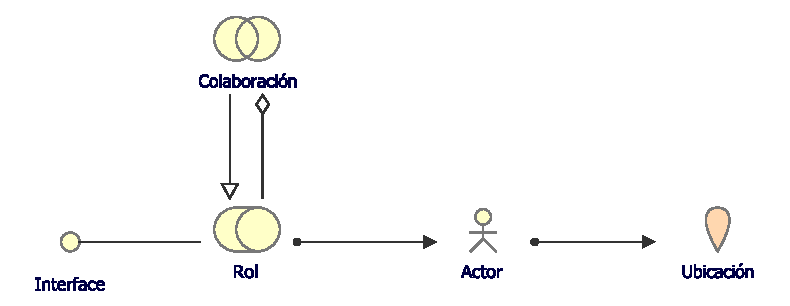
\includegraphics[width=1\linewidth]{ARQUITECTURA/imgs/MOrganizacion}
	\caption{Modelo de Ogranización}
\end{figure}


\newpage
\subsection{Caso de Estudio}

\begin{figure}[h!]
	\centering
	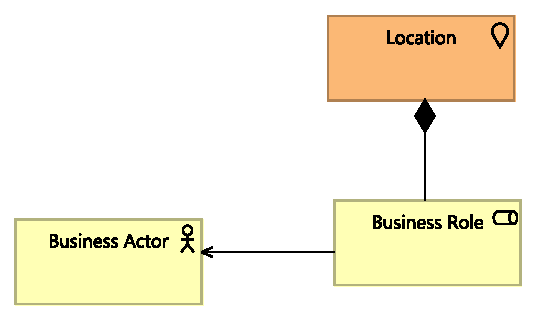
\includegraphics[width=.5\linewidth]{ARQUITECTURA/imgs/COrganizacion1}
	\caption{Modelo de Ogranización}
\end{figure}
Explicacmos nuestro caso de estudio
\newpage
%---------------------------------
\section{Punto de Vista de Fcunión de Negocio}
\subsection{Modelo}
The Organization viewpoint focuses on the (internal) organization of a company, a department, a network of companies, or of another organizational entity. It is possible to present models in this viewpoint as nested block diagrams, but also in a more traditional way, such as organizational charts. The Organization viewpoint is very useful in identifying competencies, authority, and responsibilities in an

\begin{figure}[h!]
	\centering
	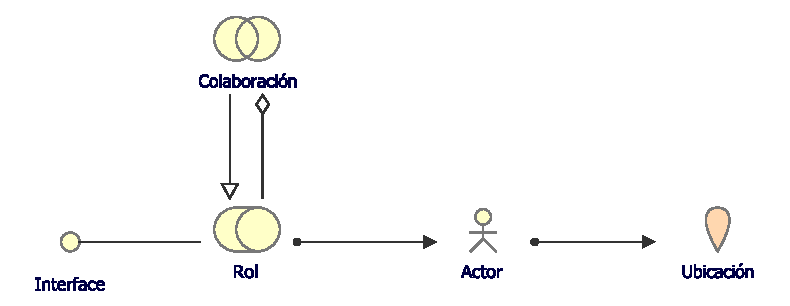
\includegraphics[width=1\linewidth]{ARQUITECTURA/imgs/MOrganizacion}
	\caption{Modelo de Ogranización}
\end{figure}


\newpage
\subsection{Caso de Estudio}

\begin{figure}[h!]
	\centering
	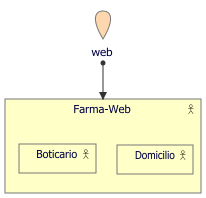
\includegraphics[width=.5\linewidth]{ARQUITECTURA/imgs/COrganizacion}
	\caption{Modelo de Ogranización}
\end{figure}
Explicacmos nuestro caso de estudio
\newpage
%---------------------------------
\section{Punto de Vista de Proceso de Negocio}
\subsection{Modelo}
The Organization viewpoint focuses on the (internal) organization of a company, a department, a network of companies, or of another organizational entity. It is possible to present models in this viewpoint as nested block diagrams, but also in a more traditional way, such as organizational charts. The Organization viewpoint is very useful in identifying competencies, authority, and responsibilities in an

\begin{figure}[h!]
	\centering
	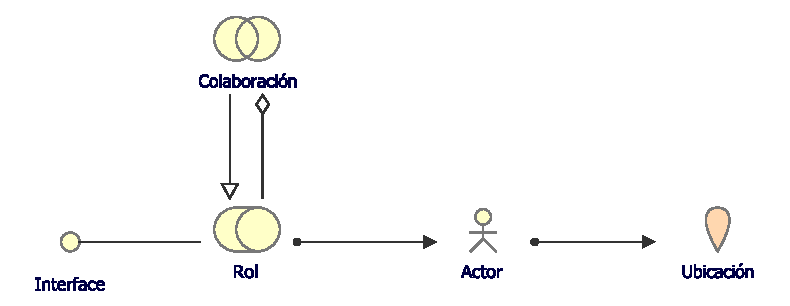
\includegraphics[width=1\linewidth]{ARQUITECTURA/imgs/MOrganizacion}
	\caption{Modelo de Ogranización}
\end{figure}


\newpage
\subsection{Caso de Estudio}

\begin{figure}[h!]
	\centering
	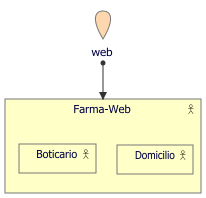
\includegraphics[width=.5\linewidth]{ARQUITECTURA/imgs/COrganizacion}
	\caption{Modelo de Ogranización}
\end{figure}
Explicacmos nuestro caso de estudio
\newpage
%---------------------------------
\section{Punto de Vista de Cooperación de Proceso de Negocio}
\subsection{Modelo}
The Organization viewpoint focuses on the (internal) organization of a company, a department, a network of companies, or of another organizational entity. It is possible to present models in this viewpoint as nested block diagrams, but also in a more traditional way, such as organizational charts. The Organization viewpoint is very useful in identifying competencies, authority, and responsibilities in an

\begin{figure}[h!]
	\centering
	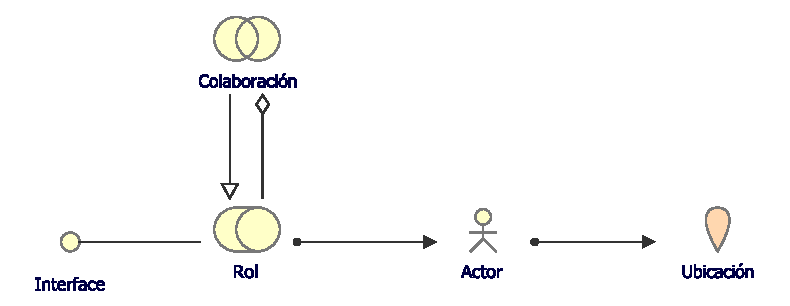
\includegraphics[width=1\linewidth]{ARQUITECTURA/imgs/MOrganizacion}
	\caption{Modelo de Ogranización}
\end{figure}


\newpage
\subsection{Caso de Estudio}

\begin{figure}[h!]
	\centering
	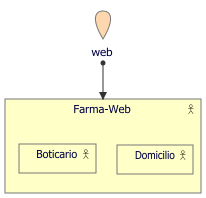
\includegraphics[width=.5\linewidth]{ARQUITECTURA/imgs/COrganizacion}
	\caption{Modelo de Ogranización}
\end{figure}
Explicacmos nuestro caso de estudio
\newpage

%---------------------------------
\section{Punto de Producto}
\subsection{Modelo}
The Organization viewpoint focuses on the (internal) organization of a company, a department, a network of companies, or of another organizational entity. It is possible to present models in this viewpoint as nested block diagrams, but also in a more traditional way, such as organizational charts. The Organization viewpoint is very useful in identifying competencies, authority, and responsibilities in an

\begin{figure}[h!]
	\centering
	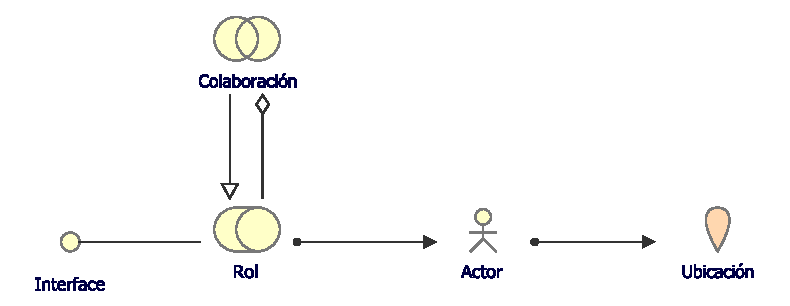
\includegraphics[width=1\linewidth]{ARQUITECTURA/imgs/MOrganizacion}
	\caption{Modelo de Ogranización}
\end{figure}


\newpage
\subsection{Caso de Estudio}

\begin{figure}[h!]
	\centering
	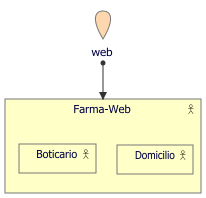
\includegraphics[width=.5\linewidth]{ARQUITECTURA/imgs/COrganizacion}
	\caption{Modelo de Ogranización}
\end{figure}
Explicacmos nuestro caso de estudio
\newpage
